\documentclass{article}
\setlength\topmargin{0pt}
\addtolength\topmargin{-\headheight}
\addtolength\topmargin{-\headsep}
\setlength\oddsidemargin{0pt}
\setlength\textwidth{\paperwidth}
\addtolength\textwidth{-2in}
\setlength\textheight{\paperheight}
\addtolength\textheight{-2in}
\usepackage{layout}
\usepackage{amsmath}
\usepackage{algorithm}
\usepackage{verbatim}
\usepackage[noend]{algpseudocode}
\usepackage{graphicx}
\graphicspath{ {./} }


\title{\vspace{-2.0cm}CS M152A Project 1 Report}
\author{Melody Chen}

\begin{document}
\maketitle
\section{Introduction and Requirement} 
The focus of this lab is for students to get used to basics of Verilog as a hardware description language and to get more familiar with the Xilinx ISE as our simulation and synthesis tool. For the first part of the project, we built a combination circuit from a diagram provided in the project specification with various gates and multiplexers. In the second part of the project, we moved on to sequential circuits and built small modules revolving around counters. We implemented 4-bit Counter in two ways, one fully based on schematics provided and one with a higher level of abstraction. For the last part, we used counters to build a simple clock divider that can be used to flash LED signal at a frequency of $1Hz$ based on a $10kHz$ clock.
\section{Design Description}
\renewcommand{\theenumi}{\alph{enumi}}
\begin{enumerate}
    \item \textbf{Combination Circuit} \\
    For this part of the project, we implemented the combination circuit below: \\
    \begin{center}
        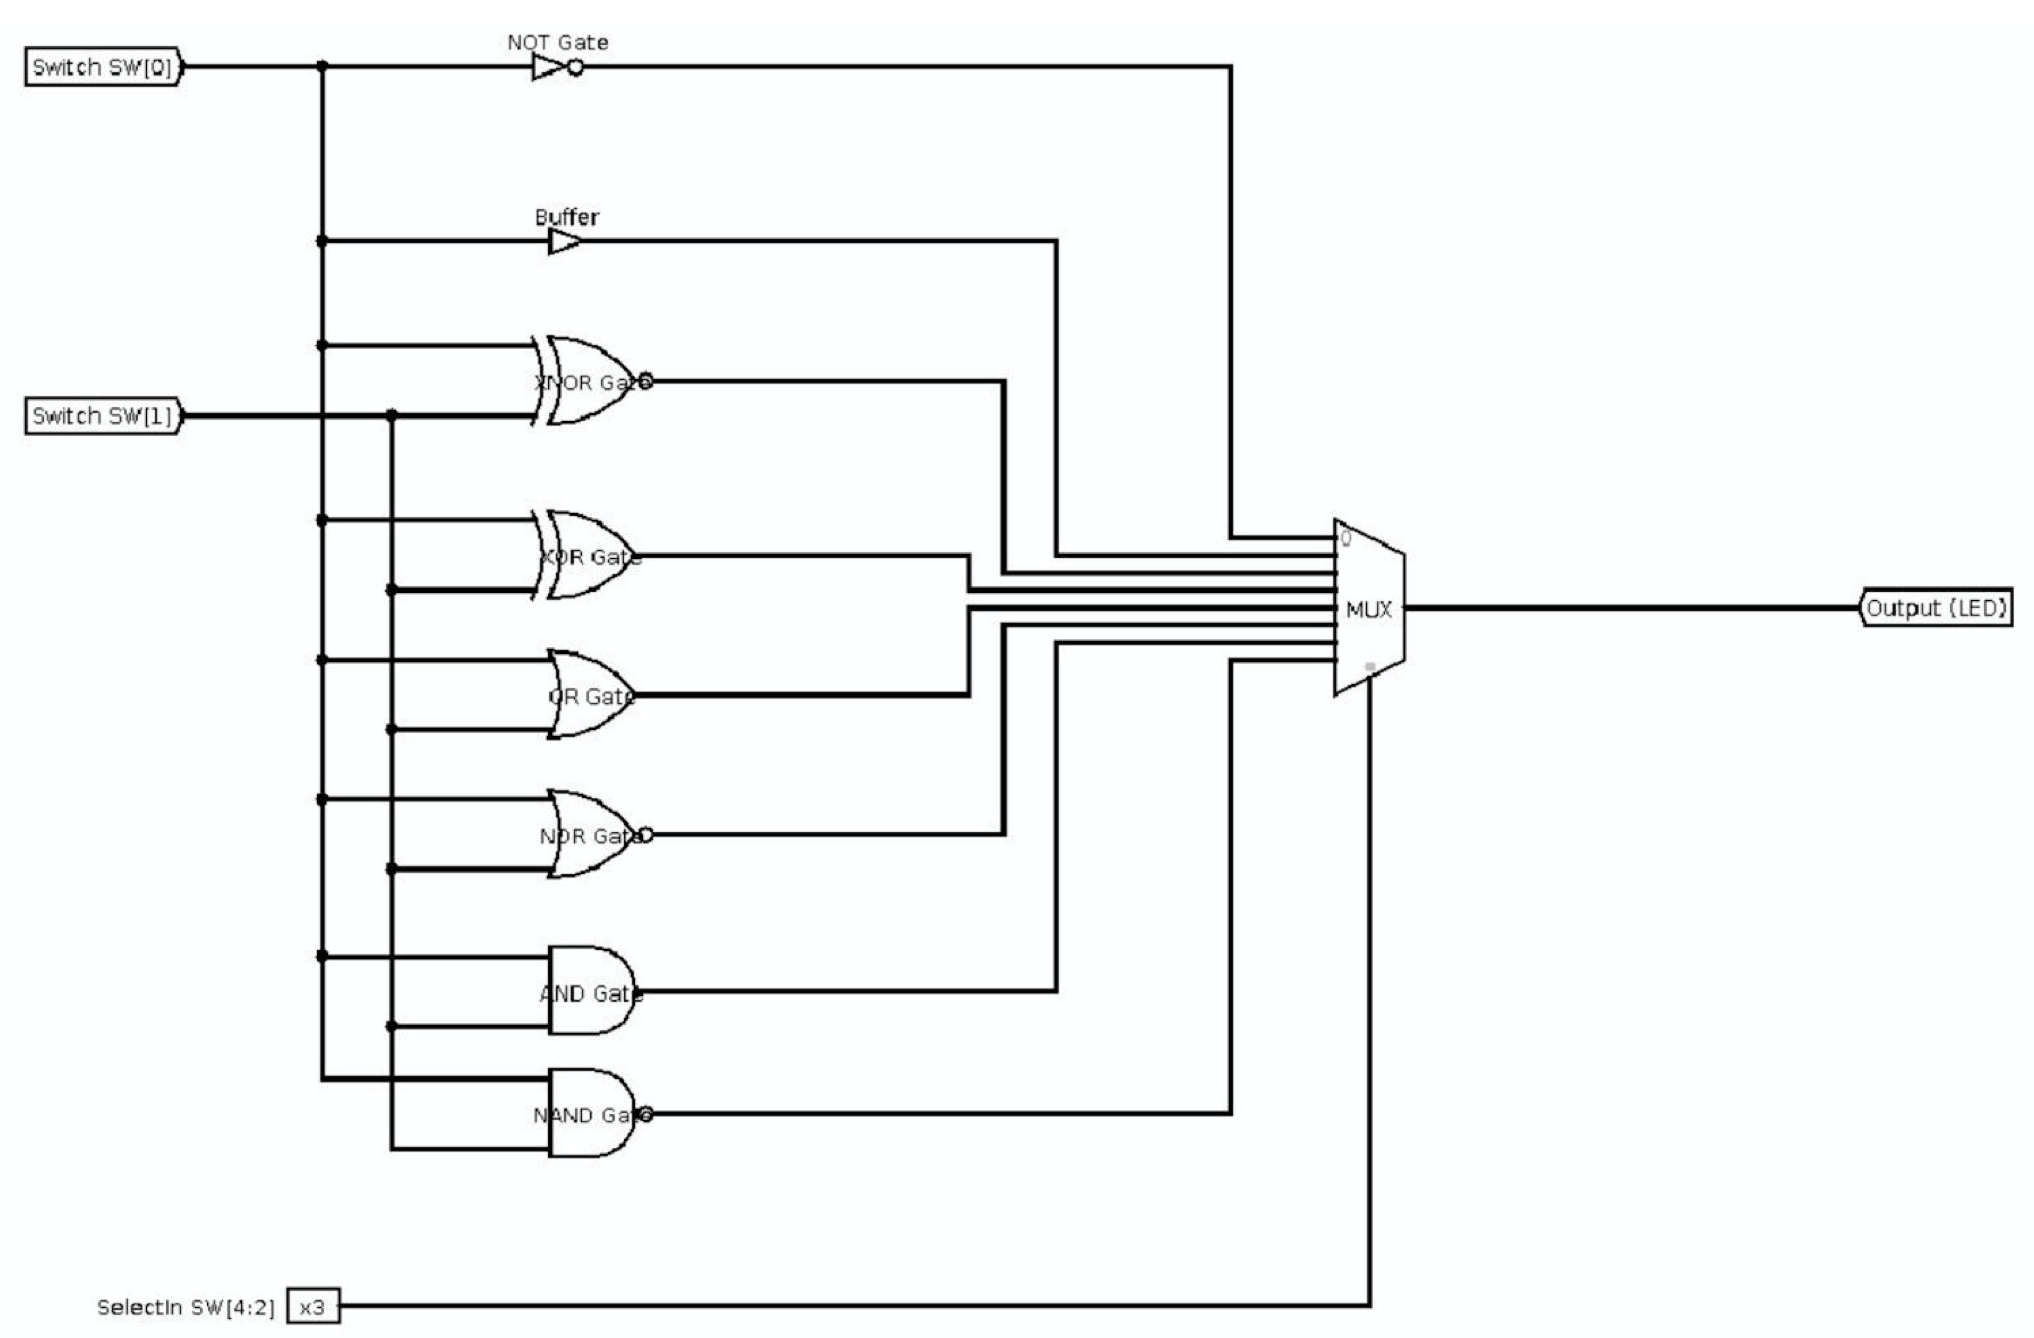
\includegraphics[scale=0.3]{ComCircuitDiagram.png} \\
        \caption{Schematic of Combination Circuit provided in Project Guidelines}
    \end{center}
    I designed one module named \texttt{CombinationCircuit} that takes in a 5-bit input \texttt{switch}, and outputs a one bit output \texttt{LED}. I used a switch statement based on \texttt{switch[4:2]} with 8 cases to implement the multiplexer. The select signal for the multiplexer comes from \texttt{switch[4:2]}. Each input into the multiplexer depends on the value of \texttt{switch[1:0]} and the operation from the circuit diagram. For example, if the select signal is \texttt{3'b111}, then we assign to \texttt{LED} the value of \texttt{$\sim$(switch[0]&switch[1])} as corresponding to select signal \texttt{3'b111} is a nand gate in the diagram above.
    \begin{center}
        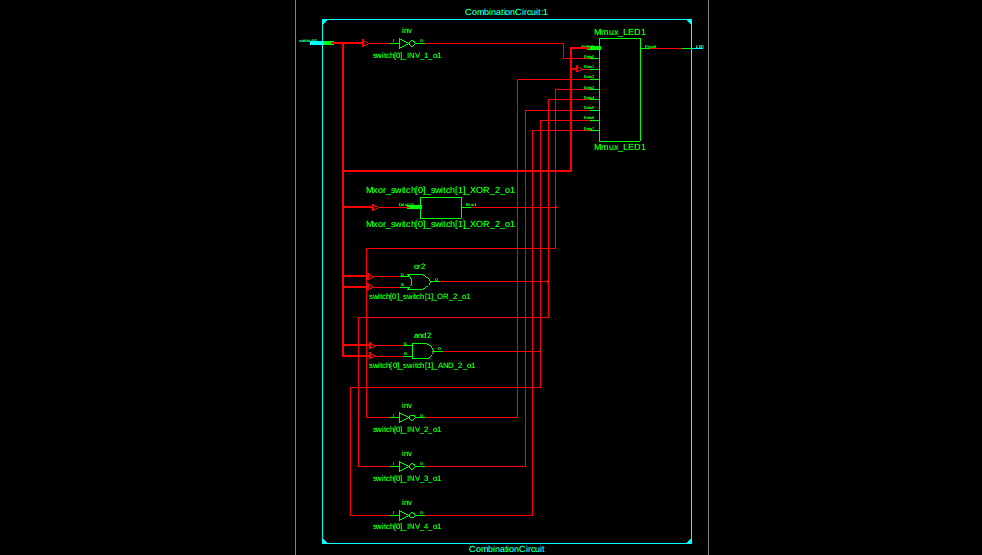
\includegraphics[scale=0.3]{combcircuitschema.png} \\
        \caption{RTL Schematic for Combination Circuit}
    \end{center}
    From the RTL schematic generated by the Xilinx ISE shown above, we can see that the hardware components in the diagram is very similar to the circuit diagram provided by the project guidelines. In the RTL schematic, different gates are used for different inputs into the multiplexer in order for different output to be computed based on the select signal.
    \item \textbf{4-Bit Counter: Translating the Schematics} \\
    For this part of the project, we designed a 4-bit counter with D flip-flops using gate-level hardware description based on the schematic below:
    \begin{center}
        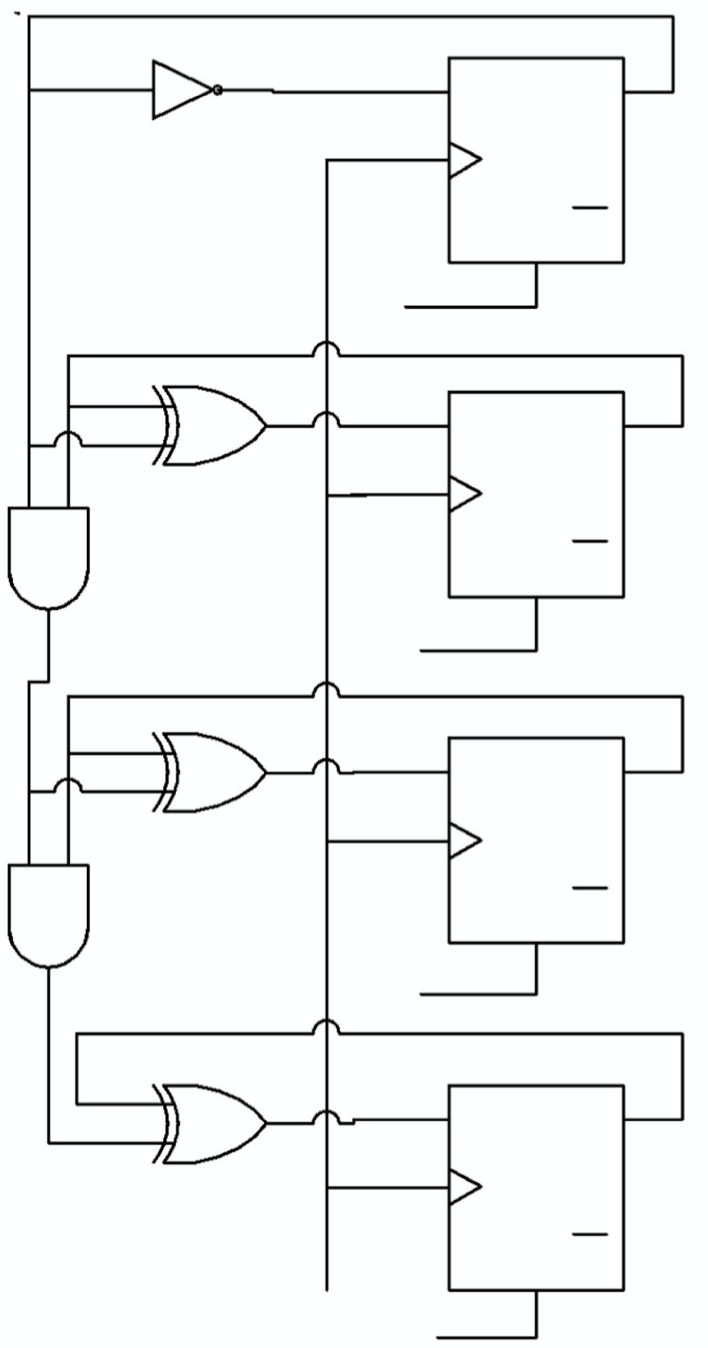
\includegraphics[scale=0.27]{SeqCircuit.png} \\
        \caption{Schematic of 4-Bit Counter provided by Project Guidelines}
    \end{center}
    I designed one module named \texttt{SeqCounter1} that takes in two 1-bit inputs \texttt{clk} and \texttt{rst}, and outputs a 4-bit output \texttt{Q} that represents the current value of the counter. Since the design of a counter is based on sequential circuits, I designed my module to have an \texttt{always} block that is triggered by \texttt{posedge clk}. Inside the \texttt{always} block, if \texttt{rst} is high, it will cause value of Q to be reset to 0. If \texttt{rst} is low, since we're translating the schematics, I map each gate to an operator and each flip-flop to a line inside the always block to execute the increment part of the counter. Thus, every time the \texttt{posedge clk} occurs, my \texttt{SeqCounter1} will increment the value of \texttt{Q} by 1 using the exact same gates and flipflops as the schematic above.
    \begin{center}
        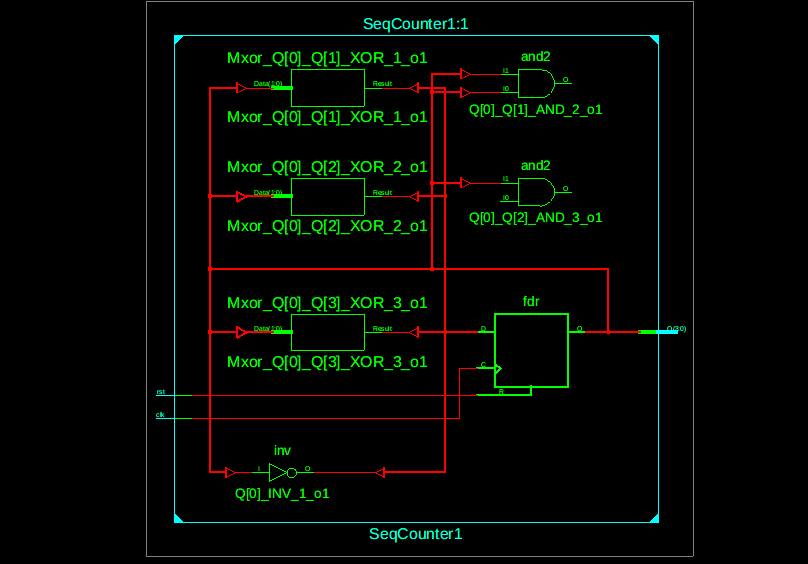
\includegraphics[scale=0.36]{seqcircuitschema1.png} \\
        \caption{RTL Schematic for 4-Bit Counter based on Schematics}
    \end{center}
    From the RTL schematic generated by the Xilinx ISE above, we can see that the hardware components used do not exactly match what is provided in the schematic in the project guidelines. Nevertheless, there are many similarities in the flip flop being used and gates being used. The two schematics are not identical even though they both accomplish the same task which is probably because Xilinx ISE tried to optimize our code for the specific FPGA we chose.
    \item \textbf{4-Bit Counter: Modern Version} \\
    For this part of the project, we created the same 4-bit counter but instead of basing the implementation directly on a schematic, we use higher level abstraction provided by Verilog HDL.\par
    I designed one module named \texttt{SeqCounterModern} that takes in two 1-bit inputs \texttt{clk} and \texttt{rst}, and outputs a 4-bit output \texttt{Q} that represents the current value of the counter. This module takes in the exact same input and output the same values as \texttt{SeqCounter1}, but the implementation varies in that instead of using gates and 4 flipflops, we use the addition operator provided by Verilog. The line \\ \texttt{Q <= Q + 1'b1} works the same way as the gates and flipflops in the schematic for \texttt{SeqCounter1}. Similar to \texttt{SeqCounter1}, the \texttt{rst} signal with an \texttt{if} statement takes care of resetting value of \texttt{Q} to 0. \par
    The modern implementation of the 4-bit Counter appears much simpler than the Schematics version, but it is important for us to be aware of the hardware underlying our Verilog code.
    \begin{center}
            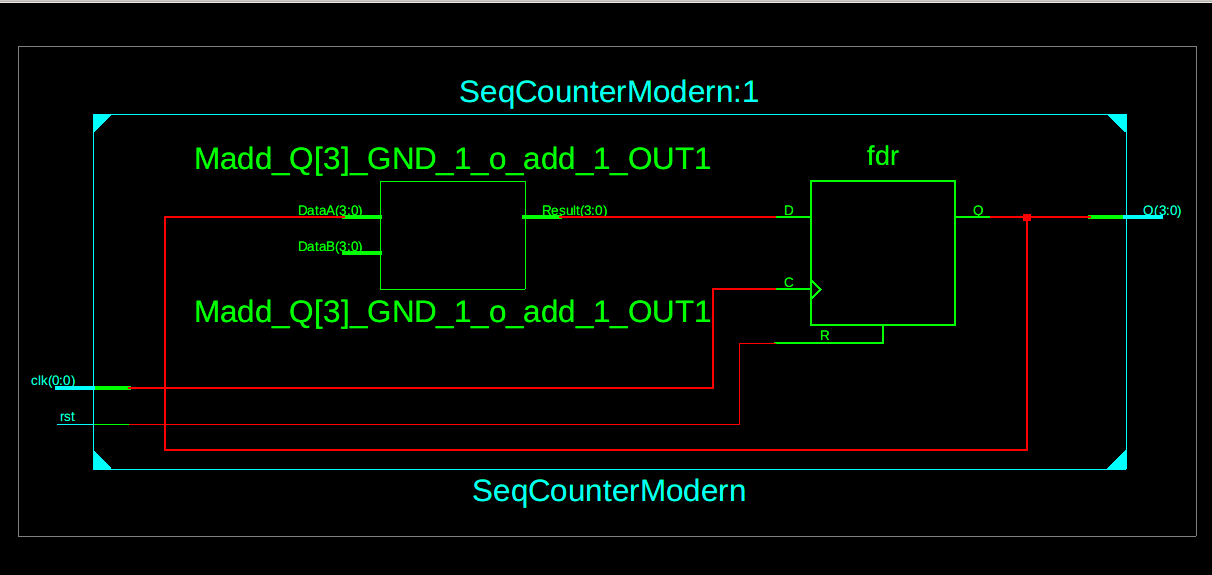
\includegraphics[scale=0.25]{seqcircuitschema2.png} \\
            \caption{RTL Schematic for Modern 4-Bit Counter}
    \end{center}
    From the RTL schematic generated by Xilinx ISE above, we can observe an adder connected to a flip flop as major hardware components. This matches our design as the \texttt{SeqCounterModern} module simply uses the \texttt{+} operator to increment output \texttt{Q} on every \texttt{posedge clk}. The \texttt{+} operator corresponds to the adder and flip flop(register) stores value of \texttt{Q} until next \texttt{posedge clk}.
    
    
    \item \textbf{Clock Divider: Counter in Action} \\
    In this part of the project, I designed and implemented clock dividers using the concept of counters. The project specified us to build a flashing LED with a frequency of $1Hz$ and in the test bench we should design and use a $10kHz$ clock. \par
    To build the divider, I created a module \texttt{clockDivider} that takes in two 1-bit signals \texttt{clk} and \texttt{rst} as inputs and outputs a 1-bit signal \texttt{out}, which should be high every 1 second. In order to keep track how much time has passed we use the \texttt{clk} signal, a 13-bit register \texttt{count}, and a local parameter \texttt{constNumber = 5000}. \texttt{constNumber} represents the value our counter will count until, it is set to 5000 as we have a $10kHz$ clock and we want the LED to flash at $1Hz$ i.e. flash every one second. Since clock is at a 10000x higher frequency than our LED flash frequency, we want signal \texttt{out} to be high every time clock hits 10000 iterations(reaches \texttt{posedge} 10000 times). We use register \texttt{count} to keep track of number of iterations clock has had a \texttt{posedge}, when \texttt{count} is 5000, this means that signal of \texttt{flash} needs to flip in order for LED to flash(\texttt{out} to be switched to high) every 1 second. Thus, our register \texttt{count} needs to be 13 bits as the highest value \texttt{count} will store is 5000 and $\log_{2}(5000)=13$.\par
    In my module, I have two \texttt{always} blocks. The first \texttt{always} block takes care of incrementing \texttt{count} and resetting \texttt{count} when \texttt{count} hits 5000 or when \texttt{rst} is high. The second \texttt{always} block takes care of flipping signal of \texttt{out} when \texttt{count} hits 5000 and keeping the signal of \texttt{out} the same at all other times or 1 when \texttt{rst} is high. \par
    With the above implementation, the \texttt{out} signal will flash(turn on) at a frequency of $1Hz$ if a clock signal of $10kHz$ is passed in as the \texttt{clk} parameter.
    \begin{center}
        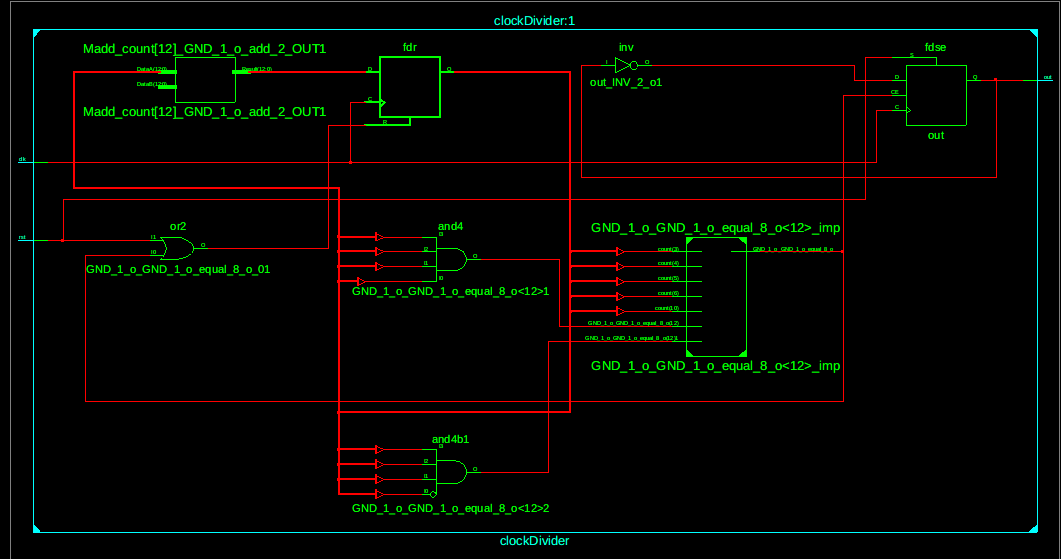
\includegraphics[scale=0.29]{seqcircuitschema3.png} \\
        \caption{RTL Schematic for Clock Divider}
    \end{center}
    From the RTL schematic generated by the Xilinx ISE above, we can see that our \texttt{clockDivider} module is more complicated than our previous three modules. We can observe registers being used to store values of \texttt{count} and output value, adder being used to increment \texttt{count}, and comparators being used to compare values of \texttt{count} and local parameter\texttt{constNumber}.
\end{enumerate}

\section{Simulation Documentation}
\begin{enumerate}
    \item \textbf{Combination Circuit} \\
    For the Combination Circuit Module, in my test bench I tested different values of \texttt{switch [4:0]} and observed how they change the value of output \texttt{LED}. For example, when \texttt{switch [4:0] = 5'b00000}, according to the schematic, the output \textttt{LED} should be the invert \texttt{switch[0]}, which should be 1. As shown in the first 100ns of the simulation waveform, when \texttt{switch [4:0] = 5'b00000}, \textttt{LED = 1}. In the next 100ns, the input \texttt{switch [4:0] = 5'b00001}, thus the output \textttt{LED} should be the invert \texttt{switch[0]}, which should be 0 and it is 0 in the simulation waveform. At 200ns, \texttt{switch [4:0] = 5'b11110}, so according to the schematics, the nand operation should be done on \texttt{switch[0], switch[1]} and should result in \textttt{LED = 1}, which matches output in waveform below.
    \begin{center}
        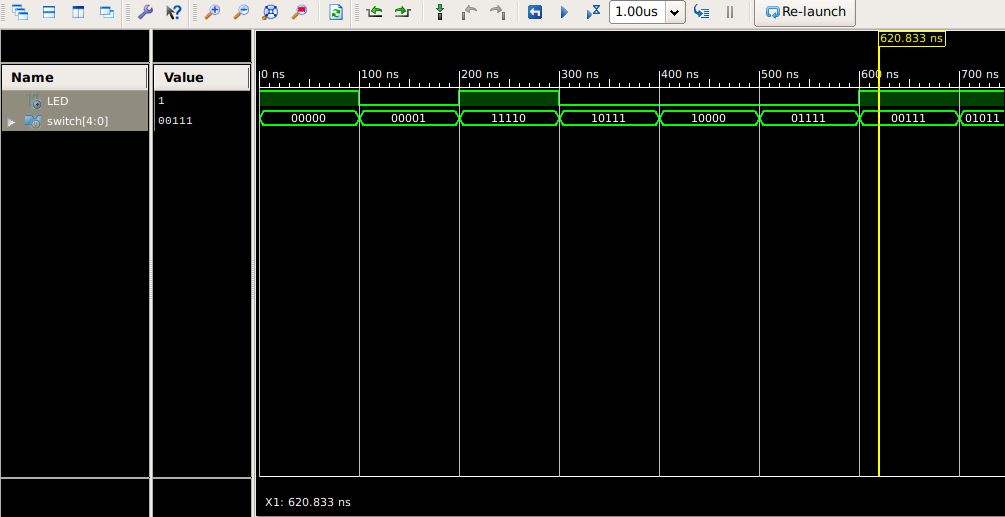
\includegraphics[scale=0.4]{tb_comb.png} \\
        \caption{Simulation Waveform for Combination Circuit}
    \end{center}
    \par
    \textbf{Synthesis and Implementation Report} included at end of document.
    
    \item \textbf{4-Bit Counter: Translating the Schematics} \\
    For this part of the project, my test bench flips the clock signal in order to trigger the \texttt{always} block to increment our 4-bit counter. A correct 4-bit counter should increment its output by 1 each time a \texttt{posedge clk} occurs. Below is the output waveform of my test bench: 
    \begin{center}
        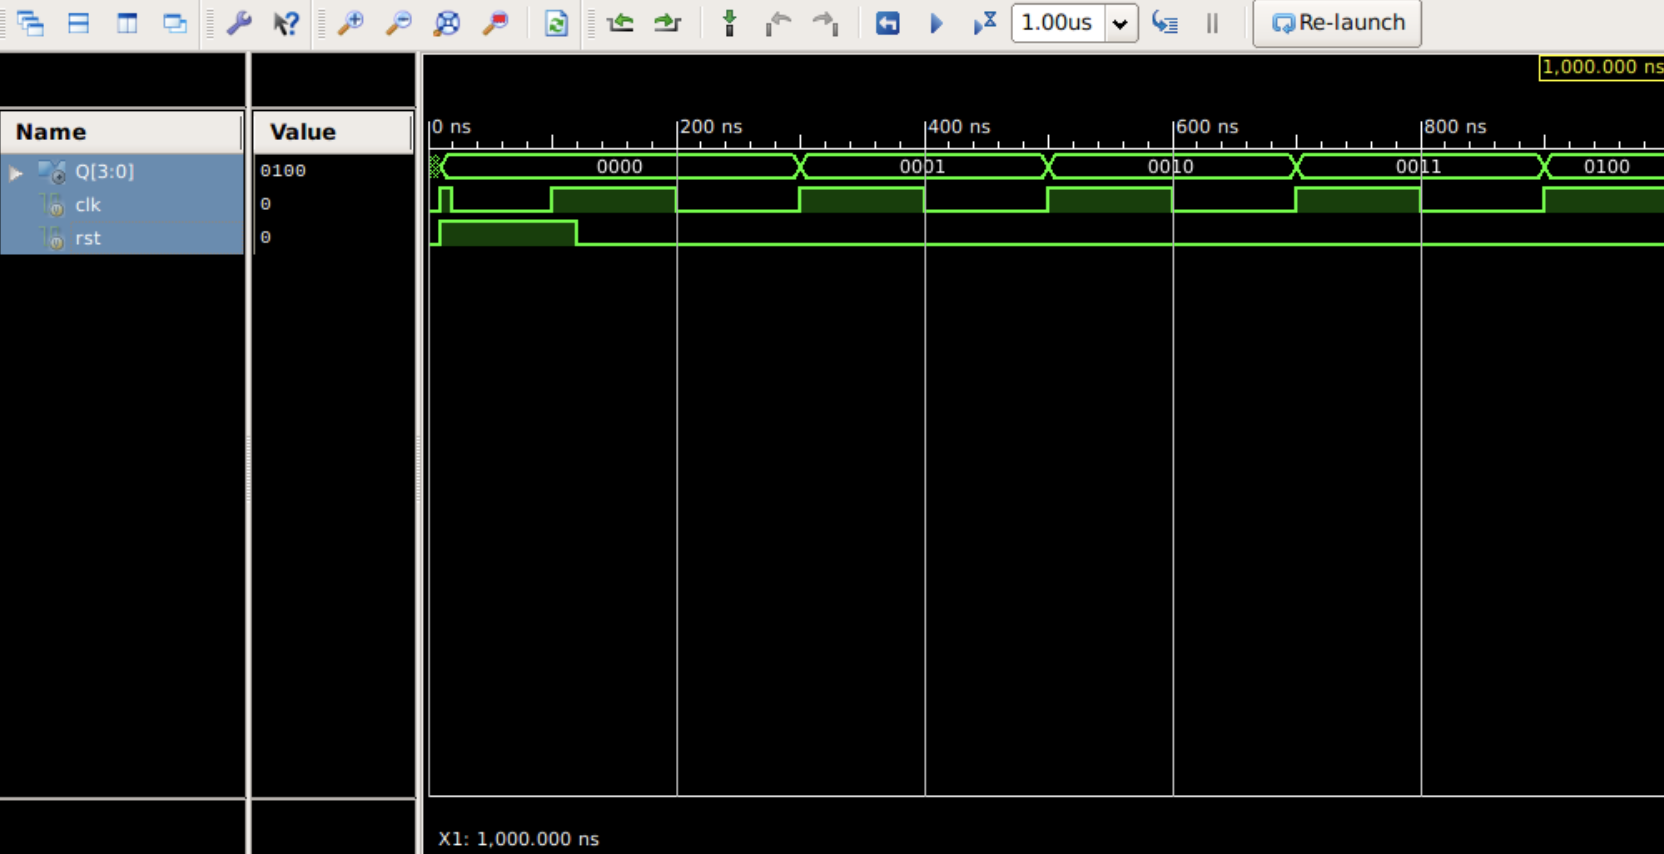
\includegraphics[scale=0.5]{tb_comb1.png} \\
        \caption{Simulation Waveform for 4-Bit Counter(Schematics)}
    \end{center}
    From the waveform diagram above, we can see that when \texttt{rst} is high and \texttt{clk} has a \texttt{posedge}, the output \texttt{Q} is set to 0. When \texttt{rst} is low and \texttt{clk} has a \texttt{posedge}, the output \texttt{Q} increments by 1 at every \texttt{posedge}. The waveform from my test bench highlights that the 4-bit counter implemented based on the schematics works as stated by the specifications. \par
    As I implemented the \texttt{SeqCounter1} module, my test bench and wave form helped me realized that early on I had a bug where my output \texttt{Q} was always \texttt{xxxx}. I realized that the reason for this error was in the start of my test bench when I set \texttt{rst} to high, it was not detected by my \texttt{always} block as I switched \texttt{rst} back to low prior to occurrence of \texttt{posedge clk}. \par
    \textbf{Synthesis and Implementation Report} included at end of document.
    
    \item \textbf{4-Bit Counter: Modern Version} \\
    My test bench for this part of the project is the same as my test bench for the schematics version of 4-Bit Counter as different implementation of 4-bit counter should receive the same outputs given the same inputs. Below is the output wave form of my test bench:
    \begin{center}
        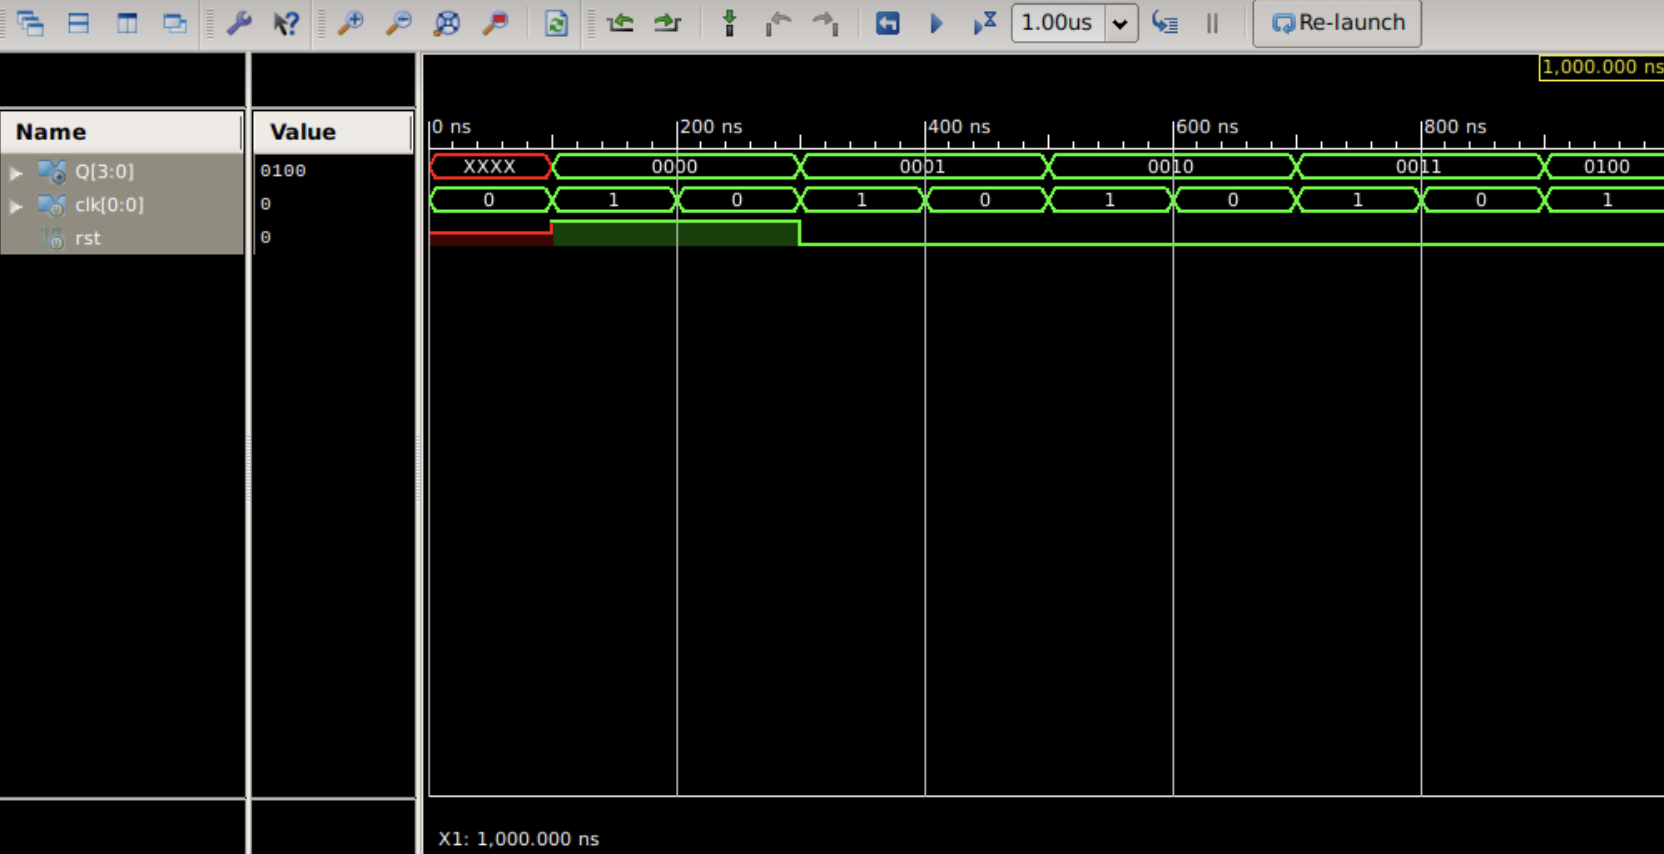
\includegraphics[scale=0.5]{tb_seq1.png} \\
        \caption{Simulation Waveform for 4-Bit Counter(Modern)}
    \end{center}
    From the diagram above, we can see that before both \texttt{rst} is high and \texttt{posedge clk} the output \texttt{Q} is \texttt{xxxx}. But after \texttt{rst} is high and \texttt{posedge clk}, the value of \texttt{Q} is correctly 0. Once \texttt{rst} is low, at every \texttt{posedge clk} output \texttt{Q} increments by 1. Thus, from the wave form diagram, we know that the modern implementation of 4-bit Counter works as specified by the project guidelines. \par
    \textbf{Synthesis and Implementation Report} included at end of document.
    \item \textbf{Clock Divider: Counter in Action} \\
    To test to see if my Clock Divider can actually flash a LED at a frequency of $1Hz$, I implemented a $10kHz$ clock in my test bench. The $10kHz$ clock is easily implemented by an \texttt{always} block that simply flips the \texttt{clk} with a 50000ns delay. With this $10kHz$ clock, our implementation of clock divider should output signal \texttt{flash} as high at a frequency of $1Hz$ i.e. once every second. \par
    The wave form from my test bench is shown below:
    \begin{center}
        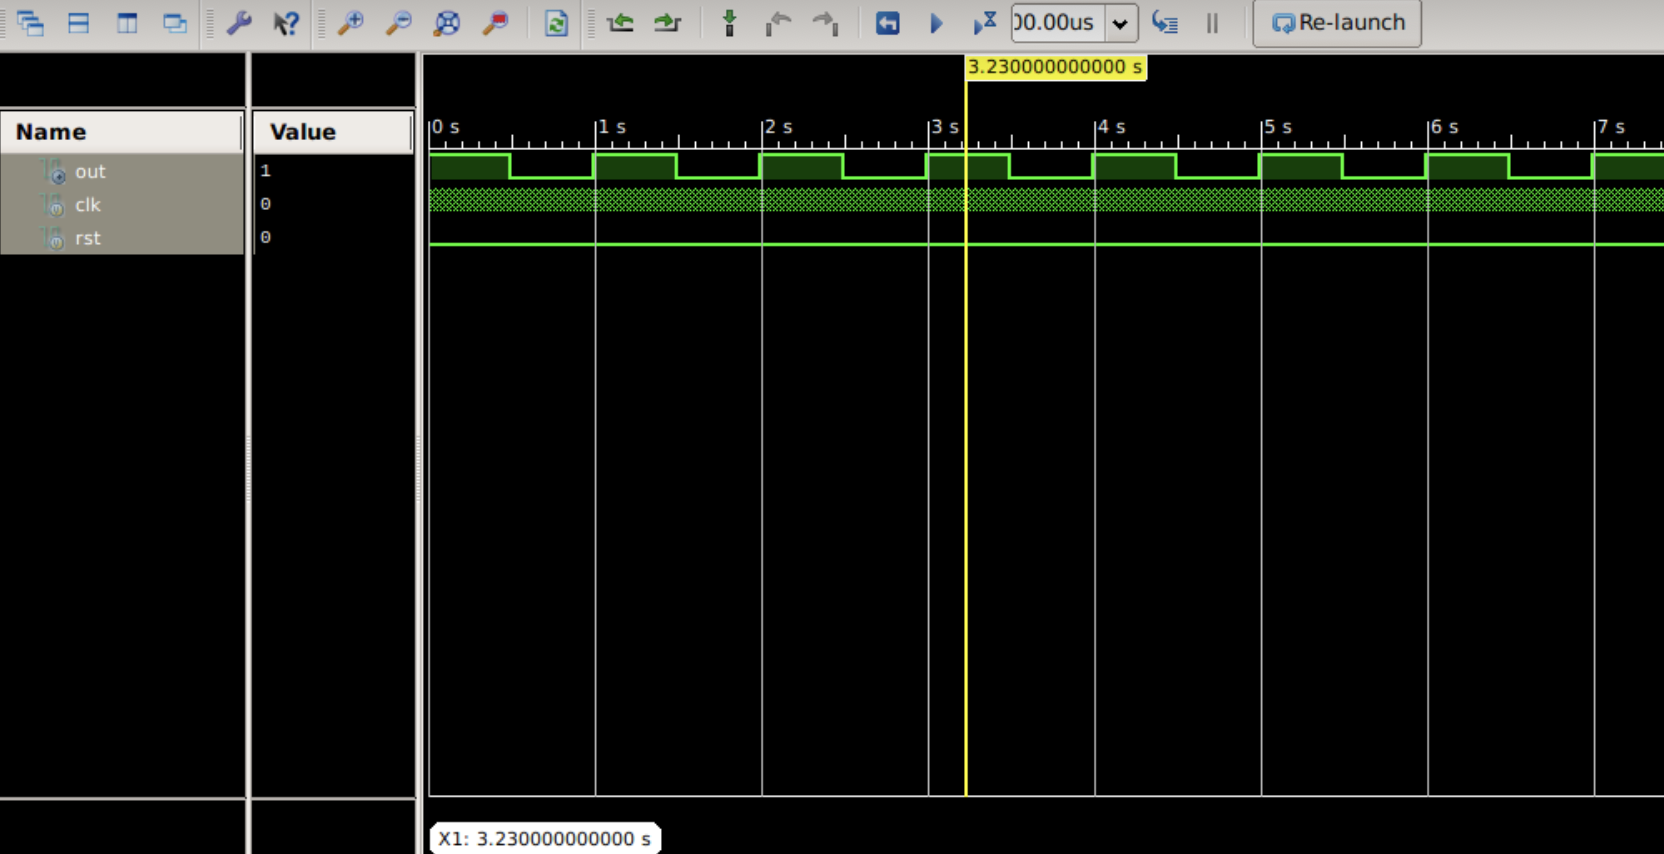
\includegraphics[scale=0.5]{tb_seq2.png} \\
        \caption{Simulation Waveform for Clock Divider}
    \end{center}
    From the diagram above, we can see that indeed every second, the output signal switches from low to high. Thus, if the output signal was an LED, it would flash at frequency of $1Hz$. \par
    One bug I encountered as I tested my module was that my output signal did not appear to change and stayed high for the entirety of the simulation. After some debugging, I realize that my simulation was not running long enough for the output signal to change. \par
    \textbf{Synthesis and Implementation Report} included at end of document.
\end{enumerate}

\section{Additional Questions} 

 What is a “.ucf” file? How would you use it for Nexys3 in an actual setting on a real board to connect the inputs of the combinational circuitry to the switches on the FPGA? \\
 \\
\textbf{Answer: } A ".ucf" file in Xilinx is a constraints file format. It helps apply constraints to the Xilinx tool, such as pin mappings and timing based on your hardware. For us, we can use it to find out information about how to connect inputs of combinational circuitry to switches on the FPGA. For example, the ".ucf" file can tell us which pins we should use to connect external hardware components that our module will interact with for Nexys3. Without the ".ucf" file, it will be extremely difficult for us to know how our Verilog module will interact with Nexys3 and its hardware components.



\section{Conclusion} 
In this project, I designed and implemented four different modules and tested each of them with its own test bench in order to gain a better understanding of Verilog and how the Xilinx ISE works. The first module is an implementation of a Combination Circuit provided by the project guidelines. It was implemented with Verilog operators and a case statement to describe a multiplexer. The second module is an implementation of a sequential 4-bit Counter based on the schematic provided. The implementation uses logic gates and 4 d flip flops, which is more complicated than the implementation in the third module. Third module implements the same 4-bit Counter but with a higher level of abstraction, directly using the plus operator provided by Verilog. The last module is a clock divider that is used to flash LED(output signal) at frequency of $1Hz$ implemented using two \texttt{always} blocks, comparators to check when signal of LED should be flipped, and concept of counter in the previous two modules. \\ \\
Some challenges I faced during this project include initializing the values of signal in test bench and navigating through various parts of the Xilinx ISE to generate different reports. I was able to overcome these difficulties by looking through notes provided by the TA and debugging through looking at the wave form diagrams.

\newpage
\small
\section{Reports}
\subsection{Synthesis Report for Combination Circuit}
\verbatiminput{combcircuit-report.txt}
\newpage
\subsection{Implementation Report for Combination Circuit}
\verbatiminput{imp-report1.txt}
\newpage
\subsection{Synthesis Report for 4-Bit Counter (Schematics)}
\verbatiminput{seqcircuit1-report.txt}
\newpage
\subsection{Implementation Report for 4-Bit Counter (Schematics)}
\verbatiminput{imp-report2.txt}
\newpage
\subsection{Synthesis Report for 4-Bit Counter (Modern)}
\verbatiminput{seqcircuit2-report.txt}
\newpage
\subsection{Implementation Report for 4-Bit Counter (Modern)}
\verbatiminput{imp-report3.txt}
\newpage
\subsection{Synthesis Report for Clock Divider}
\verbatiminput{seqcircuit3-report.txt}
\newpage
\subsection{Implementation Report for Clock Divider}
\verbatiminput{imp-report4.txt}
\end{document}